\documentclass[12pt, a4paper]{article}

\usepackage[ngerman]{babel}
\usepackage{csquotes}
\usepackage{geometry}
\usepackage{graphicx}
\usepackage{caption}
\usepackage{microtype}
\usepackage[all]{nowidow}
\usepackage[style=authoryear,backend=biber,maxcitenames=2]{biblatex}
\usepackage{fontspec}

%%%%%% Textformatierung %%%%%%%%%%%%%%%%%%%%%%%%%%%%%%%%%%%%%%%%%%%%%%%%%%%%%%%%

\setmainfont[
    Path = {fonts/},
    ItalicFont = {EBGaramond-Italic.ttf},
    BoldFont   = {Charter-Bold.ttf},
]{EBGaramond.ttf}

\setlength{\parskip}{0.5em} % Abstand zwischen Absätzen
\setlength{\parindent}{0cm} % Absätze sollen nicht eingerückt werden

% Seitenränder
\geometry{bindingoffset=1cm, left=3cm, right=3cm}

%%%%%% Abbildunggen %%%%%%%%%%%%%%%%%%%%%%%%%%%%%%%%%%%%%%%%%%%%%%%%%%%%%%%%%%%%

\graphicspath{{./figures/}}
\captionsetup{width=0.8\linewidth} % Abbildungen sind 80% der Textbreite
\setkeys{Gin}{width=0.8\linewidth} % ... und Bildunterschriften auch

%%%%%% Zitate und Quellenverweise %%%%%%%%%%%%%%%%%%%%%%%%%%%%%%%%%%%%%%%%%%%%%%

% Es gibt mehrere Befehle, mit denen Zitate in ein Latex-Dokument einfügen
% werden können. Angenommen, es gibt einen 'newton1833' Eintrag in der .bib
% Datei und ich möchte ... , dann kann das folgende Befehl verwendet werden.
%
%     ... indirekt zitieren:
%         \vglcite{80f}{newton1833} => (vgl. Newton 1687, S. 80f)
%
%     ... eine Textpassage aus dem Ausgangstext übernehmen:
%         \verbcite{150}{newton1833} => (Newton 1687, S. 150)
%
%     ... eine Bildquelle einfügen:
%         \verbcite{95}{newton1833} => (Newton 1687, S. 95)
%
%     ... auf das gesamte Werk verweisen:
%         \autocite{newton1833} => (Newton 1687)
%
%     ... nur den Titel der Arbeit haben:
%         \citetitle{newton1833} => Philosophiæ Naturalis Principia Mathematica
%

\bibliography{bibliography.bib}
\newcommand{\vglcite}[2]{\autocite[vgl.][S. #1]{#2}}
\newcommand{\verbcite}[2]{\autocite[][S. #1]{#2}}

% Quellenverweise sollen nicht mit einem Punkt beendet werden.
\renewcommand*{\finentrypunct}{}

% Abkürzung o.D. (ohne Datum) soll für Webseiten verwendet werden, für die kein
% Datum in der .bib Datei eingetragen wurde.
\DeclareLabeldate{
    \field{date}\field{eventdate}\field{origdate}\field{year}\literal{nodate}
}

% Seitenränder von Blockzitaten
\renewcommand{\quote}{
    \list{}{\rightmargin=2em\leftmargin=2em\topsep=0em}\item\relax\small
}

% Abbildungsverzeichnis soll nicht extra eingerückt werden.
\makeatletter
\renewcommand{\l@figure}{\@dottedtocline{1}{0em}{2em}}
\makeatother

%%%%%% Ende der Prä­am­bel %%%%%%%%%%%%%%%%%%%%%%%%%%%%%%%%%%%%%%%%%%%%%%%%%%%%%

\begin{document}

\begin{titlepage}
    \centering
    \Large
    \newgeometry{bindingoffset=1cm}

    \vspace*{\fill}
    
    {\Huge\textbf{Titel der Arbeit}\par}
    \vspace{0.5cm}
    {\LARGE\textbf{Untertitel}}
    
    \vspace{3cm}
    
    Vorwissenschaftliche Arbeit verfasst von\par
    \textbf{Max Mustermann}\par
    
    \vspace{1.5cm}
    
    Klasse: 8B\par
    Schuljahr: 2020/21\par
    
    \vspace{1.5cm}
    
    Betreuer: \textbf{Prof. Mag. Thomas Mustermann}\par
    
    \vspace{3cm}
    
    Bundesrealgymnasium Wien 4\par
    Waltergasse 7\par
    1040 Wien
    
    \vspace*{\fill}
\end{titlepage}

\pagestyle{empty}
\setcounter{page}{2}
\section*{Abstract}
\addcontentsline{toc}{section}{Abstract}

Quae consequatur autem. Consequatur et natus neque ea dolorem magni. Dolorum culpa voluptas. Quis distinctio qui magni debitis maiores. Officia quia necessitatibus at tenetur voluptatibus tempora quidem sed adipisci. Veniam modi laudantium quod dolore et ex deserunt molestiae ut. Omnis saepe totam eius esse accusamus ullam. Enim ut officiis nesciunt et explicabo aut reiciendis possimus. Veritatis totam iure voluptates autem eos quia reprehenderit aperiam sit. Quia quo accusamus nostrum perspiciatis. Occaecati incidunt nemo quae et sed. Asperiores consequatur quia tempora. Officiis tempore consequatur voluptas optio eos deserunt.

% Inhaltsverzeichnis
\newpage
\pagestyle{empty}
\tableofcontents
\newpage
\pagestyle{plain}

\section{Einleitung}

Eum non enim molestiae voluptatem sed animi nobis labore illum. Accusantium non neque et. Ea nam iste explicabo voluptatum aliquam tempore et aut inventore. Et deserunt deserunt delectus dolorum maxime officia et assumenda qui. Fugiat hic rerum sed est praesentium. Vero maiores aut explicabo quas ut veritatis laudantium. Incidunt aut cupiditate sunt accusamus suscipit repellendus autem perspiciatis. Commodi sed iste voluptas qui omnis. Fugit accusantium quisquam error. Non et rerum sint neque. Pariatur incidunt optio minima reprehenderit aut sint voluptate omnis eum.

Sed non lorem dolor. Proin ultricies purus sit amet justo vestibulum, ac vehicula ante imperdiet. Nulla egestas non lorem sit amet rhoncus. Fusce accumsan quam lorem, quis lacinia lectus eleifend in. Donec finibus ante ut pulvinar eleifend. Fusce ut tortor dictum, interdum elit non, eleifend diam. Nunc tristique ullamcorper nibh, ac efficitur eros pulvinar egestas. Maecenas finibus quam at luctus auctor. Duis diam ante, porta non lorem in, viverra eleifend dui.

\section{Dignissimos dicta magnam\label{sec:kapitel_mit_abbildung}}

In seinem Werk \citetitle{newton1833} formuliert der Autor \citeauthor{newton1833} die drei Grundgesetze der Bewegung. Außerdem wird in diesem Buch das Gesetz der Schwerkraft hergeleitet, das Anziehungskräfte zwischen allen Körpern beschreibt.

Fusce tristique volutpat elementum. Aenean elementum nibh ex, et consectetur augue ultricies tristique. Ut hendrerit blandit orci, ut varius dolor vehicula in. Proin malesuada sagittis quam, quis iaculis nibh venenatis sit amet. Vivamus interdum eros eu egestas varius. Duis ut massa pretium, luctus metus id, ultricies sapien. Fusce volutpat risus arcu, non vehicula velit fermentum vel. Curabitur in porta dolor, ac viverra metus. Morbi sit amet velit vitae libero bibendum pretium. Integer pellentesque, dui vel finibus posuere, turpis urna placerat odio, in fringilla elit nisi eu lacus. Etiam tempus mattis augue vitae eleifend. Mauris cursus magna arcu. Lorem ipsum dolor sit amet, consectetur adipiscing elit. Nunc tempor enim a varius iaculis.

\begin{quote}
    If Carroll was on drugs, the Alice books would probably be a series of rambling, disconnected, surrealist scenarios. But the Alice books are far from random. They contain some very intricate logic problems and very clever puns (not to mention Alice’s journey in “Through the Looking-Glass”, which follows the moves of a chess game), that could only be the work of a sharp mind in full control of its abilities. \autocite{rooy_faq}
\end{quote}

Labore incidunt aliquam tenetur et. Dolorem dolor et et est. Et sit unde aliquid eligendi quia consectetur aliquam totam. Culpa minima error est perferendis voluptatem nulla est molestias nesciunt. Illum minima hic laudantium optio dolor omnis. Est quaerat quaerat delectus natus quos laboriosam. Libero iure perferendis itaque. Repellat in quaerat inventore sed nobis et et. Fugiat deleniti fuga sit beatae. Sit illum odit autem nisi quaerat et aut. Enim sint provident expedita est blanditiis tempore minima sapiente. Quo saepe aspernatur tempore.

\subsection{Dolor excepturi ratione}

Deleniti sed laudantium et et. Est et magnam quasi qui. Ratione ipsum voluptatem harum cupiditate nihil sit dolor numquam. Quasi at est. Eum reprehenderit id nihil. Qui pariatur id sed enim. Provident cupiditate voluptatum est temporibus aut qui quidem tempore corporis. A mollitia excepturi. Praesentium sed vitae beatae et temporibus qui. Qui vero ad optio inventore. Quo assumenda et facilis aut quod consequuntur provident. Aut illo quo quasi sint earum possimus voluptate sit asperiores. In et id libero quia qui repudiandae et. Commodi numquam quaerat. Et quos non rerum laboriosam nulla. Quia tenetur mollitia.

Nulla nec nibh molestie, faucibus augue at, tristique ipsum. Vestibulum dapibus sapien eu arcu cursus, vel iaculis eros consectetur. Phasellus dolor dui, varius id iaculis nec, laoreet vel nisl. Sed consequat ullamcorper facilisis. Fusce viverra molestie ipsum non placerat. In in ligula a turpis hendrerit bibendum. Nulla quis lorem ornare, volutpat elit at, fermentum tellus. Aliquam sollicitudin, arcu vitae faucibus blandit, nisi velit cursus ex, eu lobortis tellus turpis id diam. Curabitur quam enim, molestie tempus molestie at, porttitor quis risus. Mauris egestas ornare massa, non condimentum nisi.

\begin{figure}
    \centering
    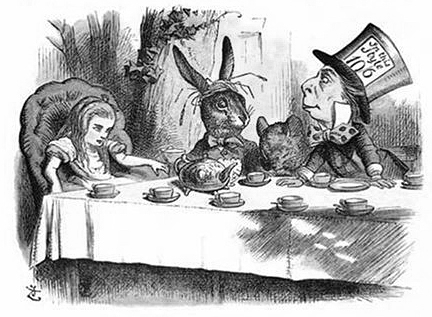
\includegraphics{alice}
    \caption{Alice bei einer Teegesellschaft im Wunderland \verbcite{33}{carroll1865}}
    \label{fig:teaparty}
\end{figure}

Die Abbildung \ref{fig:teaparty} zeigt Alice bei einer Teeparty mit dem Märzhasen und dem verrückten Hutmacher. Die beiden Gastgeber stützen ihre Ellbogen auf ein Murmeltier, das fest eingeschlafen zwischen den beiden liegt. Die Protagonistin Alice bemerkt, dass diese Lage unbequem für das Tier sein müsse \vglcite{33f}{carroll1865}.

\subsection{Rerum dolores inventore}

Magnam consequatur cum quis ut et quos quo molestiae. Reiciendis quia et magnam fugit eos aperiam ut velit ea. Repudiandae animi tempore. Qui aut ut ex vero voluptatibus. Non illum voluptatem enim et. Vitae quisquam in quo molestiae voluptatem incidunt. Qui nostrum rerum fugiat nihil soluta repudiandae commodi. Sunt doloribus omnis deleniti aperiam suscipit. Perspiciatis qui aspernatur sed fuga dolores qui sed. Ipsam excepturi quis est possimus dolores temporibus optio illum. Voluptatem odio aut modi voluptate nihil ipsam. Nesciunt sequi tempore quos laudantium blanditiis ipsam totam labore. Dolores ab reiciendis aut pariatur. Et quo non nihil quia et cum ullam vitae voluptas. Distinctio architecto quis quasi necessitatibus ea.

Cumque deleniti ut et ex nobis. Consectetur ut voluptas fuga deleniti rerum itaque praesentium libero facilis. Consequuntur ut exercitationem nobis. Iusto tempora voluptatem architecto quidem voluptatum repellat. Quisquam laboriosam adipisci in ex. Odio ad rerum dolores autem quo eius autem sequi. Accusamus dolores sunt ad provident ab fugit vel natus. Quas laborum animi et quibusdam itaque et omnis. Consequuntur labore ut in nisi non sed ratione. Consequatur et quis. Ut dolores assumenda aliquam sint nulla ipsam quia voluptas. Possimus in et dicta.

\begin{itemize}
    \item Alice
    \item Cheshire Cat
    \item White Rabbit
    \item Queen of Hearts
\end{itemize}

Dolore voluptatibus dolores incidunt commodi id. Est fuga non sapiente similique est. Totam suscipit animi dolor voluptate qui amet consequatur. Deleniti expedita perspiciatis quo quos ut est culpa sint. Quos omnis modi perferendis aut deleniti sint cum autem. Recusandae consequuntur et ut natus quaerat vitae qui magnam.Accusamus et sapiente laborum eum repudiandae facere id. Ipsam eum modi unde tempore enim qui omnis consequatur. Aut eum perferendis. Aliquid est repellat quia architecto vel minima quibusdam.

\section{Explicabo consequature}

\begin{figure}
    \centering
    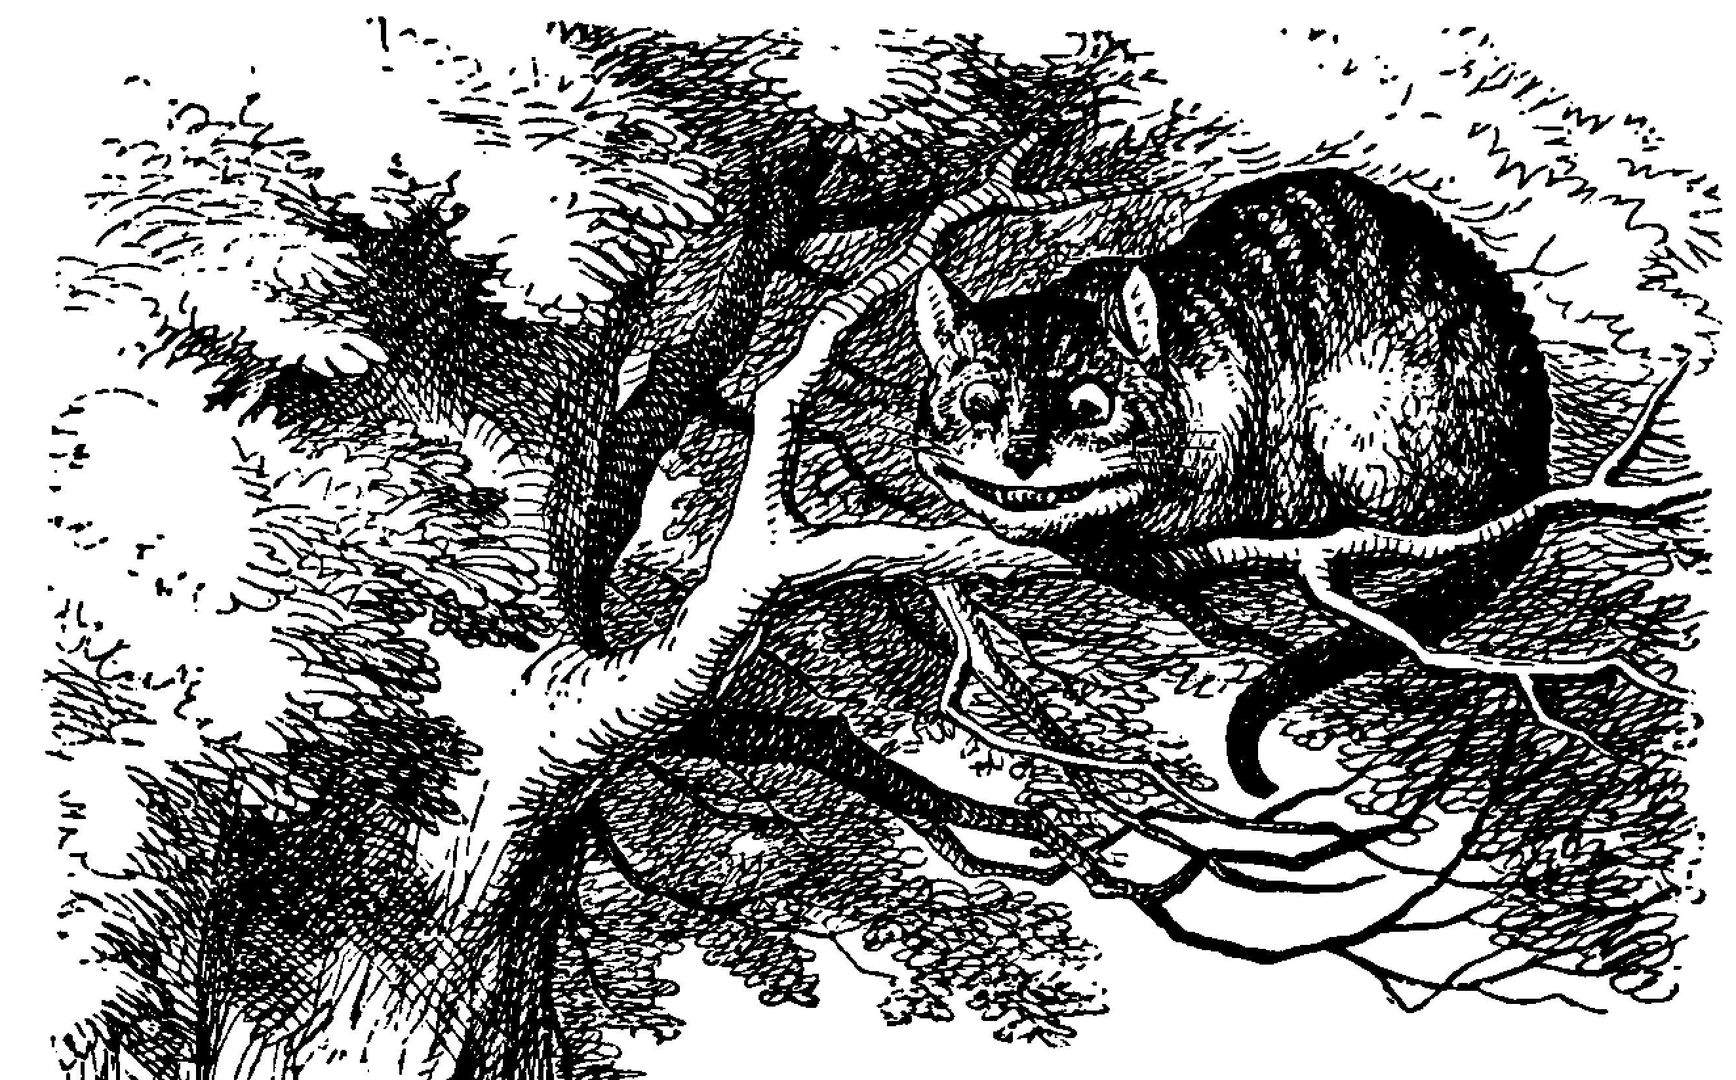
\includegraphics{cheshire_cat}
    \caption{Große Grinsekatze auf einem Baum \verbcite{31}{carroll1865}}
    \label{fig:fat_cat}
\end{figure}

Die Abbildung \ref{fig:fat_cat} zeigt eine große und etwas übergewichtete Katze, die auf einem Baum sitzt und mit Alice spricht. Die Katze grinst, weil sie mit ihrem Leben im Wunderland vollständig zufrieden ist. Außerdem meint die Grinsekatze, dass alle Lebewesen, die im Wunderland leben und später Alice begegnen werden, verrückt sind. Die Abbildung der Grinsekatze stammt aus dem Buch \citetitle{carroll1865}, das im Jahr \citeyear{carroll1865} von \citeauthor{carroll1865} geschrieben wurde \autocite{carroll1865}.

Integer non purus tellus. Nulla nec tellus dictum, lacinia magna quis, luctus velit. Sed elementum tristique pulvinar. Proin congue tincidunt dapibus. Nam nisl lacus, cursus nec lobortis eu, pretium in leo. Proin ultricies diam sit amet lorem sodales sagittis. Fusce molestie congue mi at lacinia. Nunc faucibus id urna et volutpat. Aenean tempus sit amet lacus a luctus. Fusce sit amet scelerisque odio. Sed et tortor sollicitudin, blandit turpis non, viverra ipsum. Donec varius mollis dui eget commodo. Sed quis nisl pharetra, vestibulum felis dictum, iaculis felis. In id justo mauris. Proin nec enim ullamcorper, convallis felis vel, sagittis mi. Fusce ut dui lacus.

\section{Zusammenfassung}

Im Kapitel \ref{sec:kapitel_mit_abbildung} wurden viele Absätze geschrieben, die überhaupt keinen Sinn ergeben und nur als Beispiele dienen. Außerdem wurde ein Bild in dieses Kapitel eingefügt, welches die Abenteuer von Alice besser veranschaulichen soll.

Curabitur eget augue imperdiet, pellentesque justo et, viverra lacus. Sed accumsan felis at maximus tempus. Duis ut elementum nibh, facilisis rutrum ex. Mauris malesuada, ipsum et aliquam vulputate, purus quam pretium elit, quis molestie nisl erat in tellus. In ultrices rutrum hendrerit. Fusce consectetur lacinia felis, eu laoreet leo scelerisque quis. Nulla sodales volutpat nulla, in faucibus massa ullamcorper id. In tempor ligula vitae feugiat vulputate. Sed fringilla posuere mauris, et tincidunt ipsum tempus malesuada. Sed semper pellentesque dictum. Curabitur urna sapien, gravida eu dapibus quis, gravida eu lacus. Mauris posuere at arcu vitae commodo.

Integer a venenatis ante, nec venenatis lacus. Quisque euismod lacinia massa eget ullamcorper. Praesent ut est faucibus, accumsan nibh ac, ornare nibh. Fusce efficitur tincidunt tellus, sed finibus ipsum. Nam rutrum sem non elit gravida suscipit. Nullam hendrerit purus vitae est euismod, quis tristique augue dictum. Donec ultrices aliquet eros, imperdiet faucibus tellus euismod ut. Aenean posuere laoreet eros a fringilla. Vivamus et vehicula orci, vel ultricies ante.

% Literaturverzeichnis
\clearpage
\printbibliography[heading=bibintoc]

% Abbildungsverzeichnis
\clearpage
\listoffigures
\addcontentsline{toc}{section}{\listfigurename}

\clearpage
\thispagestyle{empty}
\section*{Selbstständigkeitserklärung}

Ich, Max Mustermann, erkläre hiermit eidesstattlich, dass ich diese vorwissenschaftliche Arbeit selbstständig und ohne Hilfe Dritter verfasst habe. Insbesondere versichere ich, dass ich alle wörtlichen und sinngemäßen Übernahmen aus anderen Werken als Zitate kenntlich gemacht und alle verwendeten Quellen angegeben habe.

\vspace{0.5cm}
\makebox[5cm]{\hrulefill} \hfill\makebox[5cm]{\hrulefill}
\par\makebox[5cm][l]{Ort, Datum} \hfill\makebox[5cm][l]{Unterschrift}

\end{document}
